\documentclass[tikz,border=20pt]{standalone}
\usepackage{amsmath,amssymb}
\usepackage{tikz}
\usetikzlibrary{arrows.meta,calc}

\begin{document}
	
	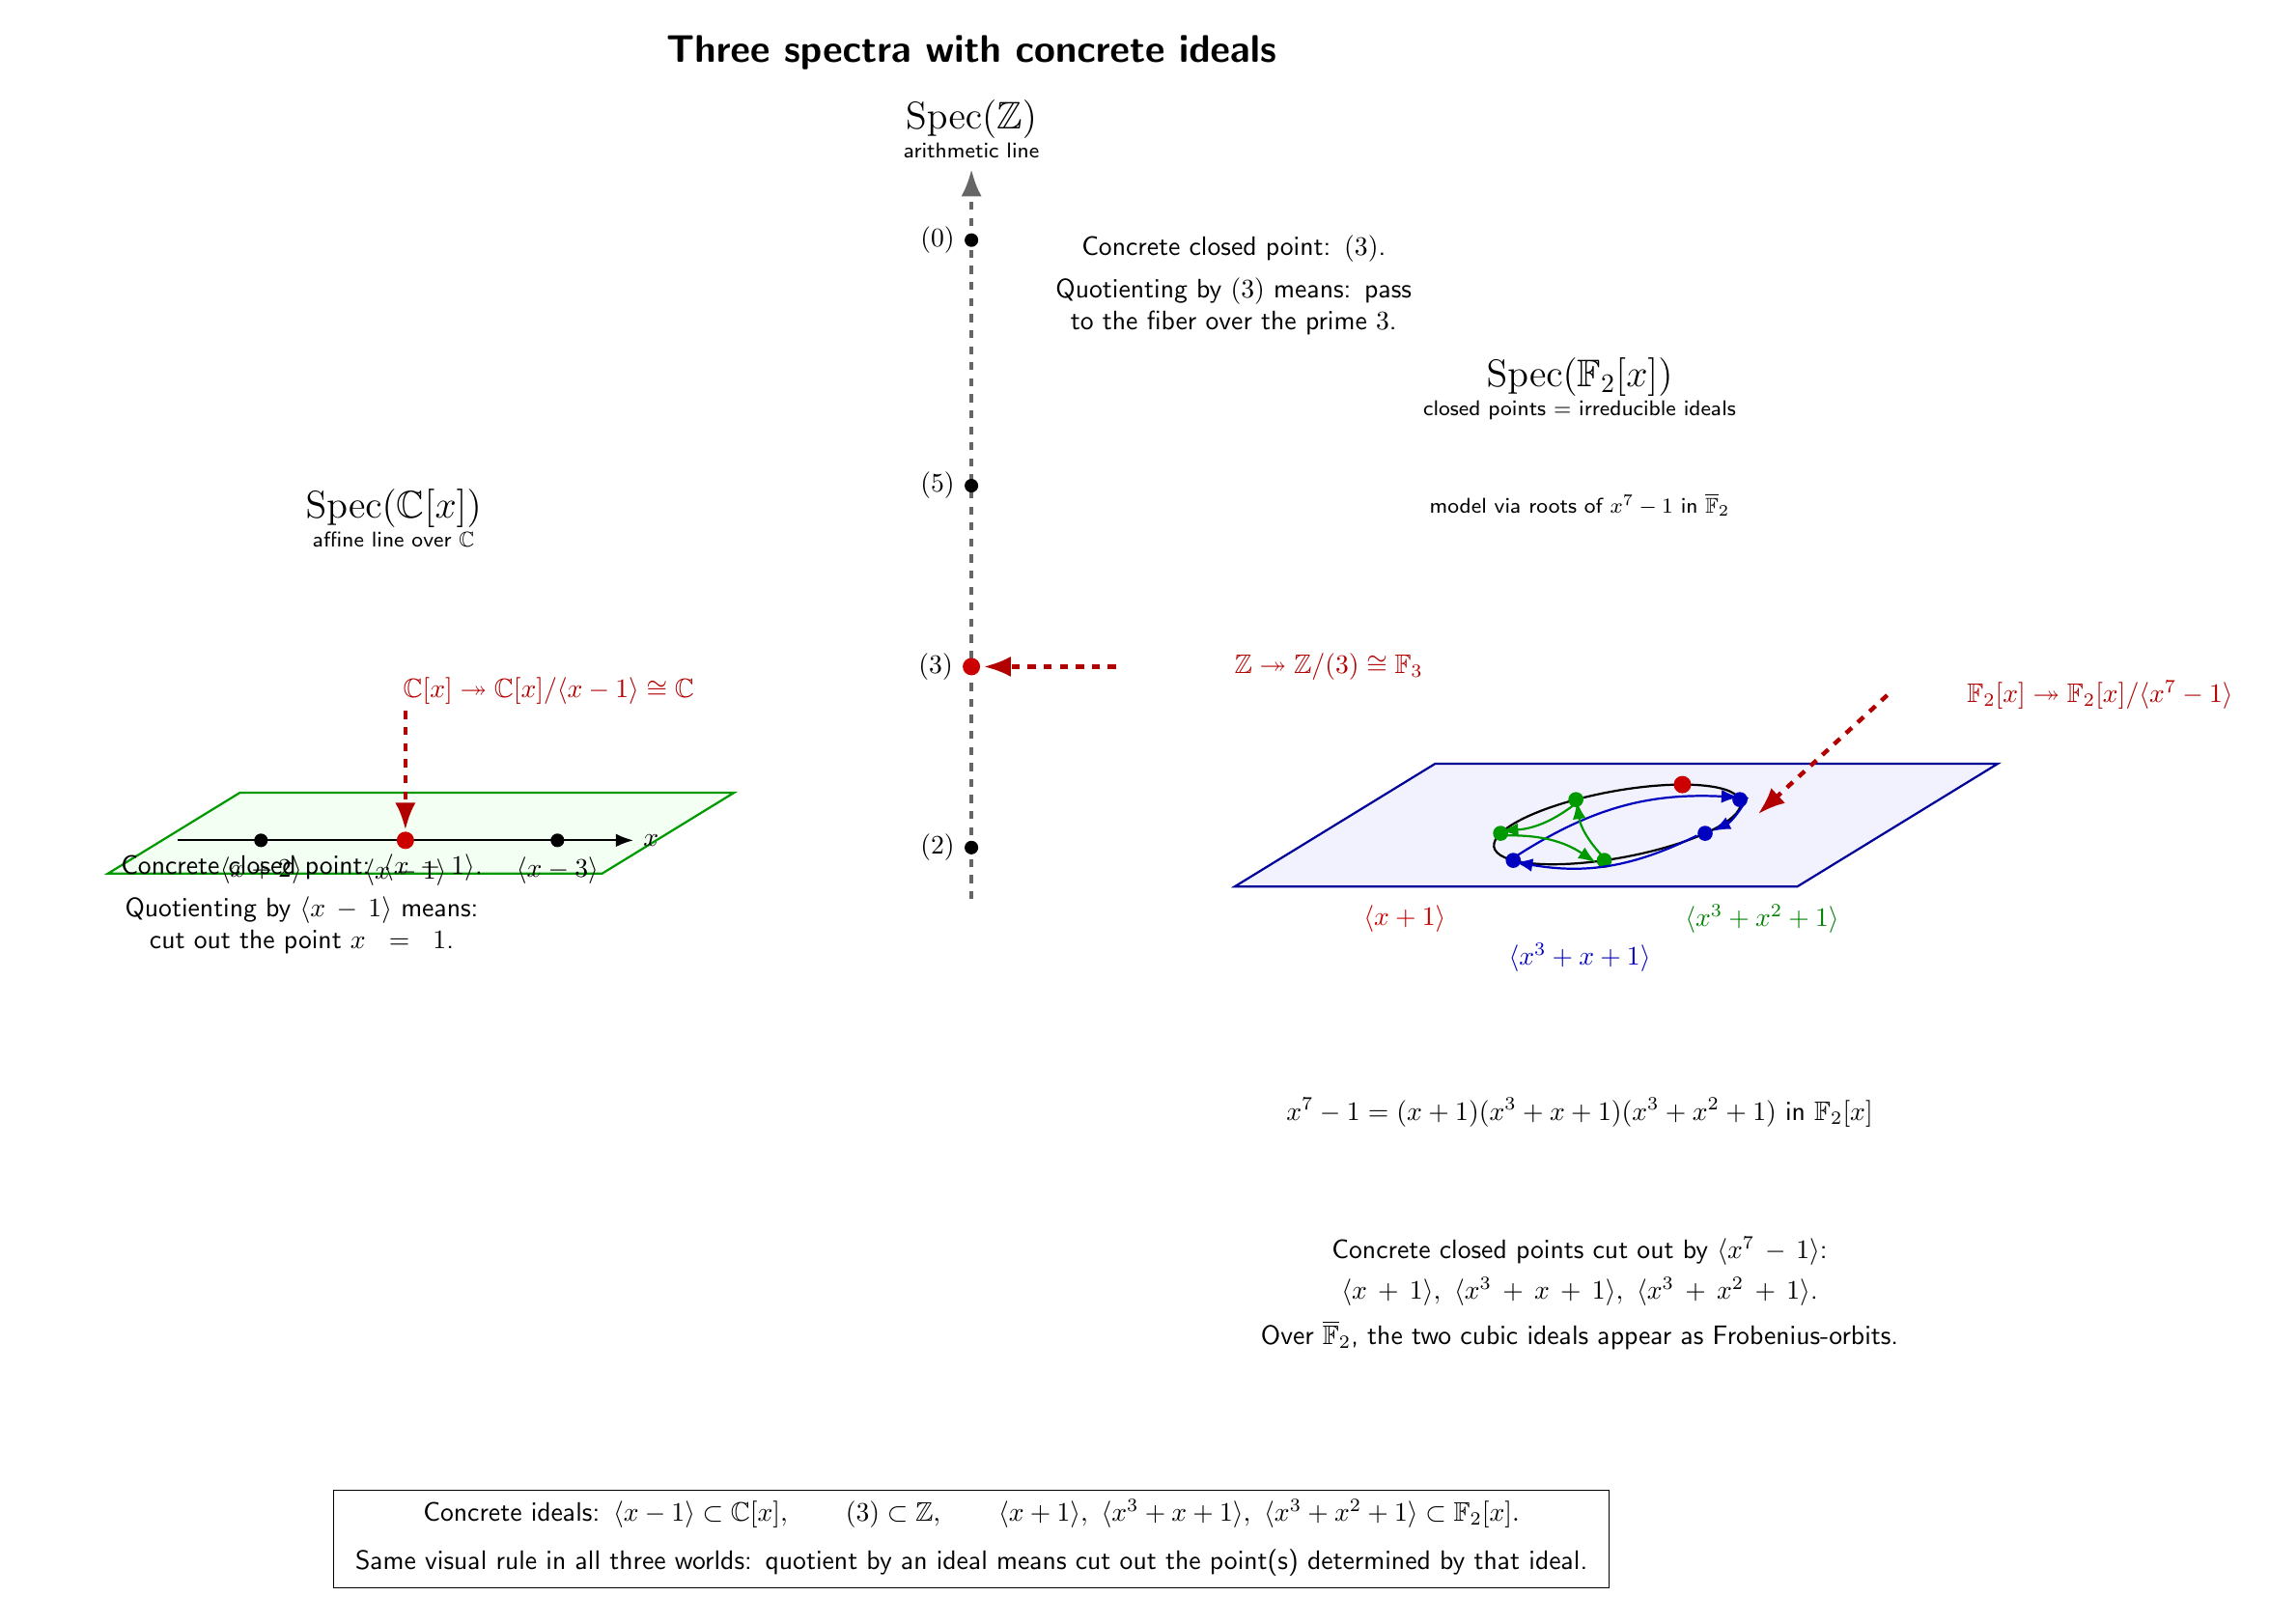
\begin{tikzpicture}[
		x={(1cm,0cm)},
		y={(0.62cm,0.38cm)},
		z={(0cm,1.7cm)},
		scale=1.0,
		font=\sffamily,
		>=Latex,
		pt/.style={circle, fill=black, inner sep=1.8pt},
		sel/.style={circle, fill=red!80!black, inner sep=2.3pt},
		orbA/.style={circle, fill=blue!75!black, inner sep=2.0pt},
		orbB/.style={circle, fill=green!60!black, inner sep=2.0pt}
		]
		
		% =========================================================
		% Global title
		% =========================================================
		\node[align=center] at (0,0,6.15)
		{\Large\bfseries Three spectra with concrete ideals};
		
		% =========================================================
		% LEFT PANEL: Spec(C[x])
		% =========================================================
		\begin{scope}[shift={(-7.6,0,0)}]
			
			\draw[fill=green!5, draw=green!60!black, thick]
			(-3.2,-0.9,0) -- (3.3,-0.9,0) -- (3.3,1.9,0) -- (-3.2,1.9,0) -- cycle;
			
			\node[align=center] at (0,0,2.55)
			{\Large $\operatorname{Spec}(\mathbb{C}[x])$\\[-1pt]\footnotesize affine line over $\mathbb C$};
			
			\draw[->, thick] (-3.0,0.25,0) -- (3.0,0.25,0) node[right] {$x$};
			
			\node[pt, label=below:{$\langle x+2\rangle$}] at (-1.9,0.25,0) {};
			\node[sel, label=below:{$\langle x-1\rangle$}] at (0.0,0.25,0) {};
			\node[pt, label=below:{$\langle x-3\rangle$}] at (2.0,0.25,0) {};
			
			\draw[->, ultra thick, dashed, red!70!black]
			(0.0,0.25,1.0) -- (0.0,0.25,0.08);
			
			\node[align=center, text=red!70!black] at (1.45,0.95,1.0)
			{$\mathbb C[x]\twoheadrightarrow \mathbb C[x]/\langle x-1\rangle\cong \mathbb C$};
			
			\node[align=center, text width=7.0cm] at (0,-1.95,0)
			{Concrete closed point: $\langle x-1\rangle$.\\[4pt]
				Quotienting by $\langle x-1\rangle$ means: cut out the point $x=1$.};
			
		\end{scope}
		
		% =========================================================
		% MIDDLE PANEL: Spec(Z)
		% =========================================================
		\begin{scope}[shift={(0,0,0)}]
			
			\draw[->, ultra thick, dashed, gray!80!black]
			(0,0,-0.4) -- (0,0,5.25)
			node[above, align=center, text=black]
			{\Large $\operatorname{Spec}(\mathbb Z)$\\[-1pt]\footnotesize arithmetic line};
			
			\node[pt, label=left:{$(2)$}] at (0,0,0.0) {};
			\node[sel, label=left:{$(3)$}] at (0,0,1.4) {};
			\node[pt, label=left:{$(5)$}] at (0,0,2.8) {};
			\node[pt, label=left:{$(0)$}] at (0,0,4.7) {};
			
			\draw[->, ultra thick, dashed, red!70!black]
			(1.9,0,1.4) -- (0.16,0,1.4);
			
			\node[align=left, text=red!70!black] at (4.7,0,1.4)
			{$\mathbb Z\twoheadrightarrow \mathbb Z/(3)\cong \mathbb F_3$};
			
			\node[align=center, text width=6.7cm] at (3.45,0,4.35)
			{Concrete closed point: $(3)$.\\[4pt]
				Quotienting by $(3)$ means: pass to the fiber over the prime $3$.};
			
		\end{scope}
		
		% =========================================================
		% RIGHT PANEL: Spec(F_2[x])
		% =========================================================
		\begin{scope}[shift={(7.9,0,0)}]
			
			\draw[fill=blue!5, draw=blue!60!black, thick]
			(-3.6,-1.35,0) -- (3.8,-1.35,0) -- (3.8,2.9,0) -- (-3.6,2.9,0) -- cycle;
			
			\node[align=center] at (0.1,0,3.55)
			{\Large $\operatorname{Spec}(\mathbb F_2[x])$\\[-1pt]\footnotesize closed points = irreducible ideals};
			
			% root circle
			\coordinate (O) at (0.1,0.8,0);
			\draw[thick] (O) circle (1.38);
			
			\node at (0.1,0,2.65) {\footnotesize model via roots of $x^7-1$ in $\overline{\mathbb F}_2$};
			
			\coordinate (P0) at ($(O)+(90:1.38)$);
			\coordinate (P1) at ($(O)+(38.571:1.38)$);
			\coordinate (P2) at ($(O)+(-12.857:1.38)$);
			\coordinate (P3) at ($(O)+(-64.286:1.38)$);
			\coordinate (P4) at ($(O)+(-115.714:1.38)$);
			\coordinate (P5) at ($(O)+(-167.143:1.38)$);
			\coordinate (P6) at ($(O)+(141.429:1.38)$);
			
			% one linear factor and two cubic factors
			\node[sel] at (P0) {};
			\node[orbA] at (P1) {};
			\node[orbA] at (P2) {};
			\node[orbA] at (P4) {};
			\node[orbB] at (P3) {};
			\node[orbB] at (P5) {};
			\node[orbB] at (P6) {};
			
			\draw[->, thick, blue!75!black]
			($(P1)+(0.05,0.08)$) to[bend left=18] ($(P2)+(0.05,0.08)$);
			\draw[->, thick, blue!75!black]
			($(P2)+(-0.06,-0.08)$) to[bend left=18] ($(P4)+(0.06,-0.06)$);
			\draw[->, thick, blue!75!black]
			($(P4)+(-0.05,0.08)$) to[bend left=18] ($(P1)+(-0.06,0.08)$);
			
			\draw[->, thick, green!60!black]
			($(P3)+(-0.05,0.08)$) to[bend left=18] ($(P6)+(0.05,-0.06)$);
			\draw[->, thick, green!60!black]
			($(P6)+(0.05,0.08)$) to[bend left=18] ($(P5)+(-0.05,0.08)$);
			\draw[->, thick, green!60!black]
			($(P5)+(0.05,-0.08)$) to[bend left=18] ($(P3)+(-0.06,-0.08)$);
			
			% concrete ideals written downstairs
			\node[align=center, text=red!80!black] at (-2.2,0,-0.55) {$\langle x+1\rangle$};
			\node[align=center, text=blue!75!black] at (0.1,0,-0.85) {$\langle x^3+x+1\rangle$};
			\node[align=center, text=green!50!black] at (2.5,0,-0.55) {$\langle x^3+x^2+1\rangle$};
			
			\node[align=center, text width=7.8cm] at (0.1,0,-2.05)
			{$\displaystyle x^7-1=(x+1)(x^3+x+1)(x^3+x^2+1)$ in $\mathbb F_2[x]$};
			
			\draw[->, ultra thick, dashed, red!70!black]
			(3.65,0.8,1.0) -- (1.95,0.8,0.08);
			
			\node[align=left, text=red!70!black] at (6.45,0.8,1.0)
			{$\mathbb F_2[x]\twoheadrightarrow \mathbb F_2[x]/\langle x^7-1\rangle$};
			
			\node[align=center, text width=8.6cm] at (0.1,0,-3.45)
			{Concrete closed points cut out by $\langle x^7-1\rangle$: \\[3pt]
				$\langle x+1\rangle,\ \langle x^3+x+1\rangle,\ \langle x^3+x^2+1\rangle$.\\[5pt]
				Over $\overline{\mathbb F}_2$, the two cubic ideals appear as Frobenius-orbits.};
			
		\end{scope}
		
		% =========================================================
		% Bottom summary
		% =========================================================
		\node[align=center, text width=17cm] at (0,0,-5.35)
		{$\boxed{
				\begin{array}{c}
					\text{Concrete ideals: }\langle x-1\rangle \subset \mathbb C[x],\qquad (3)\subset \mathbb Z,\qquad
					\langle x+1\rangle,\ \langle x^3+x+1\rangle,\ \langle x^3+x^2+1\rangle \subset \mathbb F_2[x].
					\\[6pt]
					\text{Same visual rule in all three worlds: quotient by an ideal means cut out the point(s) determined by that ideal.}
				\end{array}
			}$};
		
	\end{tikzpicture}
	
\end{document}